% !TEX root = ../../main.tex

La simulation numérique fut introduite dès l’émergence de l’informatique pour enrichir les connaissances scientifiques dans des contextes où l’expérimentation est trop contraignante voire impossible. La simulation peut aussi avoir un intérêt prédictif pour dimensionner un problème physique (simulation de tokamak avant leur construction dans le projet ITER) ou pour tester un modèle et le confronter aux futures observations (simulation de nébuleuses ou d’étoiles). La simulation peut être vue comme une retranscription informatique de modèles mathématiques, censés représenter des phénomènes physiques. La simulation numérique doit être représentative de la réalité. Ainsi, dans des modèles où la solution exacte est souvent hors de portée, il est nécessaire de vérifier que la transcription numérique conserve certaines propriétés mathématiques du modèle (conservation de certaines quantités physiques comme la masse ou l’énergie totale par exemple).

Un enjeu majeur de la modélisation et de la simulation est de maintenir un équilibre entre les approximations au niveau du modèle, qui permettent d’accélérer le temps de traitement et la précision des résultats.

Les modèles étudiés ici sont des modèles issus de la physique des plasmas. Un plasma désigne un gaz ionisé constitué généralement d'ions et d'électrons. Le terme plasma a été introduit par le chimiste et physicien américain Irving Lagmuir en 1928, par analogie avec le plasma sanguin. À la différence d'un gaz, constitué de particules neutres, un plasma est sensible à l'action d'un champ électromagnétique. Les particules chargées génèrent un champ électromagnétique qui agit sur les autres particules via la force de Lorentz et le principe fondamental de la dynamique de Newton. Cela permet de construire une classe de modèles dit particulaires où on s'intéresse à la trajectoire de toutes les particules :
$$
  \begin{cases}
    \dot{\vb{x}}_k(t) &= \vb{v}_k(t) \\
    \dot{\vb{v}}_k(t) &= \displaystyle\sum_{j\atop j\neq k} F_{jk}(t,\vb{x}_k(t))
  \end{cases}
$$
où $\vb{x}_k(t)$ et $\vb{v}_k(t)$ représentent respectivement la position et la vitesse au temps $t\geq0$ de la $k$-ème particule, avec $k=1,\dots,n$ où $n$ est le nombre de particules, $F_{jk}$ représente la force exercée par la particule $j$ sur $k$. La force considérée dans ce modèle peut être l'interaction coulombienne pour représenter l'interaction électrostatique entre particules, ou la force gravitationnelle pour représenter l'interaction à grande distance entre des masses. La complexité algorithmique d'une méthode de résolution de ce modèle est $\order{2^n}$, or dans le cadre de l'étude des plasmas, le nombre de particules $n$ en interaction est voisin du nombre d'Avogadro $\mathcal{N}_A\approx 6.02\cdot 10^{23}$. La résolution numérique de ce type de modèle fait souvent l'objet d'approximation à l'aide d'arbres de partitionnement de l'espace par exemple.

Pour décrire un tel système de particules, plusieurs possibilités existent. La description dite fluide, qui prend en compte les équations de la mécanique des fluides (comme les équations d’Euler ou de Navier-Stokes) peut être utilisée. Les inconnues de ces équations sont des quantités dites macroscopiques (mesurables expérimentalement) comme la densité, la vitesse moyenne ou la température qui ne dépendent que du temps $t$ et de la position $\vb{x}$. Cependant cette description suppose que le système étudié est à l’équilibre, c’est-à-dire que la répartition en vitesse des particules est maxwellienne. Or lorsque le système est parcouru par une onde de choc ou un laser, des phénomènes hors équilibre sont à prendre en compte exigeant une description plus précise. On utilise alors la description cinétique. Celle-ci manipule une fonction de distribution $f(t,\vb{x},\vb{v})$ dépendant du temps $t$, de l’espace $\vb{x}$ mais aussi de la vitesse des particules $\vb{v}$, ce qui permet de prendre en compte ces aspects hors équilibre. La complexité de description apportée par le modèle cinétique se traduit numériquement par un coût en temps de calcul et utilisation de la mémoire ; en effet la simulation s’effectue sur l'espace des phases $(\vb{x},\vb{v})$ plus le temps $t$, donc 7 dimensions au lieu de seulement 4 dimensions pour la description fluide, où les inconnues ne dépendent que de $(t,\vb{x})$. L’espace mémoire nécessaire pour stocker l'inconnue $f(\vb{x},\vb{v})$ sur une grille $100^6$ de l’espace des phases peut être estimé à 7.2\,To, alors que la description fluide ne nécessite que 7.6\,Mo sur une grille $100^3$ de l’espace. Une description cinétique n’est donc pas souhaitable sur tout le domaine d’étude si le fluide est proche de son équilibre et des optimisations sont donc envisageables dans ce type de configuration.

Nous nous intéresserons ici à des plasmas où les particules peuvent être distinguées en deux populations, une première dite \emph{froide} où les particules sont proche de l'équilibre, à une température $T_c$ ; une seconde dite \emph{chaude} où les particules conservent toute leur dynamique cinétique, à une température $T_h$. La température représente l'agitation moyenne des particules, ce profil de population peut être représenté, en une dimension, par la distribution tracée sur la figure~\ref{fig:intro:distrib}. Dans la modélisation, il peut être souhaitable de faire tendre $T_c$ vers $0$, impliquant alors de raffiner un maillage en vitesse pour capturer correctement une gaussienne avec une dizaine de points. Le rapport $\frac{T_c}{T_h}=\epsilon$ peut être vu comme un paramètre raide lorsque l'on se retrouve dans le cas $\epsilon \ll 1$, on peut alors construire un modèle fluide/cinétique en considérant les particules froides en équilibre thermique et en utilisant l'approximation de \emph{plasma froid}. Cette configuration a une justification physique, par exemple dans un tokamak lorsque l'on souhaite \emph{réchauffer} un plasma à l'équilibre par l'introduction d'une faible quantité de particules hors équilibre thermique ; un autre exemple est celui de l’excitation, par des particules du vent solaire, de plasma de la magnétosphère, générant ainsi des aurores boréales. La dérivation d'un modèle hybride nécessite d'effectuer un couplage entre l'équation cinétique de Vlasov, qui est conservée pour la dynamique des particules chaudes, une équation fluide, modélisant le comportement des particules froides, et les équations de Maxwell, permettant de décrire le comportement des champs électromagnétiques. 

\begin{figure}[h]
  \centering
  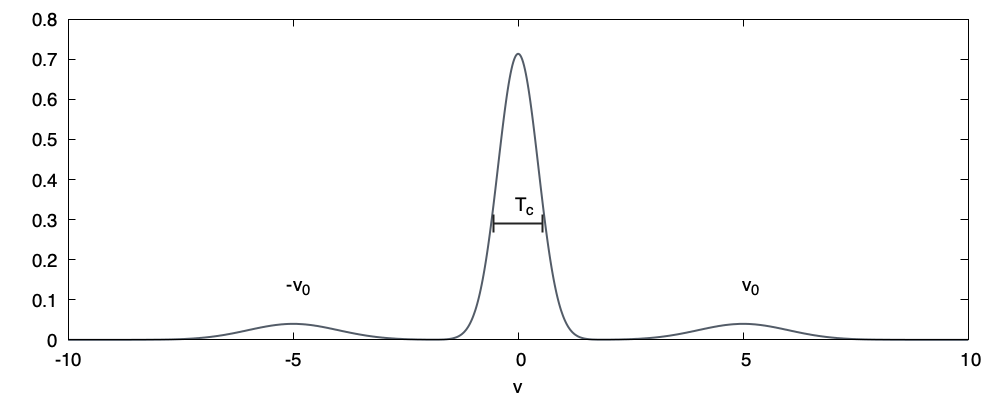
\includegraphics[width=0.9\textwidth]{\localPath/figures/distrib.png}
  \caption{Distribution en vitesse $v$ des particules en une dimension. On peut distinguer ici la population de particules froides à la température $T_c$, et la population des particules chaudes, réparties autour des vitesses $v_0$ et $-v_0$.}
  \label{fig:intro:distrib}
\end{figure}
